\documentclass{beamer}
\mode<presentation> {%
	\usetheme[]{Boadilla}
	\usecolortheme{orchid}
	\setbeamercovered{transparent}
	\setbeamersize{text margin left=0.7cm}
  \setbeamersize{text margin right=0.7cm}
  \setbeamertemplate{enumerate item}[square]
  \setbeamertemplate{enumerate subitem}[circle]
  \setbeamertemplate{enumerate subsubitem}[>]
  \setbeamertemplate{itemize item}[square]
  \setbeamertemplate{itemize subitem}[circle]
  \setbeamertemplate{itemize subsubitem}[>]
}
  
\usepackage{bm}
% \usepackage[utf8]{inputenc}
% \usepackage[spanish]{babel}
% \usepackage[normalem]{ulem}
% \usepackage{times}
\usepackage[T1]{fontenc}
\usepackage{graphicx}
\usepackage{multirow}
% \usepackage{pifont}
% \usepackage{rotating}
% \usepackage{colortbl}
% \usepackage{amssymb}

\usepackage[framed]{mcode}
\usepackage{matlab-prettifier}
\lstset{literate={ñ}{{\~n}}1}

\definecolor{olivegreen}{rgb}{0.0,0.5,0.0}
\definecolor{general}{rgb}{0.9 0.9 1}%
% \newrgbcolor{colorsistema}{0 1 1}
% \newrgbcolor{colorviolet}{0.9 0.8 1}

\title[Procesamiento de Señales]{Señales Aleatorias}
\author[Jesús Chacón Sombría] {%
 	\textit{Ingeniería Electrónica de Comunicaciones}\\
 	\vspace{0.6cm}%
	\small Jesús Chacón Sombría%
}%

\institute[DACYA. UCM] {%\inst{1}%
	\footnotesize  Departamento de Arquitectura de Computadores y Automática\\
  Universidad Complutense de Madrid
}

\date[Señales Aleatorias] % (optional)
{\footnotesize Curso 2024-2025}%{\today / Master}
\subject{Talks}

\pgfdeclareimage[height=0.75cm]{logo}{ucm}

\usepackage[absolute,overlay]{textpos}
\setlength{\TPHorizModule}{1mm}
\setlength{\TPVertModule}{1mm}
\newcommand{\MyLogo}{%
\begin{textblock}{14}(116.0,0.6)
  \pgfuseimage{logo}
\end{textblock}
}

\makeatletter
\numberwithin{section}{part}
\AtBeginPart{
\beamer@tocsectionnumber=0\relax
\frame{\partpage}
}
\makeatother

\begin{document}

\begin{frame}
  \titlepage
\end{frame}

\newcommand*\oldmacro{}%
\let\oldmacro\insertshorttitle%
\renewcommand*\insertshorttitle{%
	%\MyLogo
\oldmacro\hfill%
}

\AtBeginSection[]{}

\AtBeginSubsection[]{}



\begin{frame}\frametitle{Señales aleatorias}
  \vspace{-0.2cm}
  
  \footnotesize
  
  \begin{itemize}
    \item Una señal aleatoria ($x(t)$ ó $x[n]$)
    \begin{itemize}\footnotesize
      \item Comportamiento en cada $t$ ó $n$ definido por una v.a. $X(t)$ ó $X[n]$.
    \end{itemize}
    \item El comportamiento de la señal se puede definir a partir de:
    \begin{columns}[c]
      \begin{column}{7cm}
        \begin{itemize}
          \footnotesize
          \item La función de probabilidad conjunta
          $\color{olivegreen}p(x(0),x(1),x(2),\dots,x(10))$
          % asociada a todas$^1$ las variables asociadas a la señal aleatoria
          \item Un $\mathrm{N}^\circ$ infinito de secuencias muestrales.
          \item Los estadísticos relacionados con las v.a.
          $\color{olivegreen}\mu_{x[n]},~\phi_{x[n]x[m]}$
        \end{itemize}
        \vspace{1cm}
      \end{column}
      \begin{column}{4cm}
        \vspace{0.1cm}
        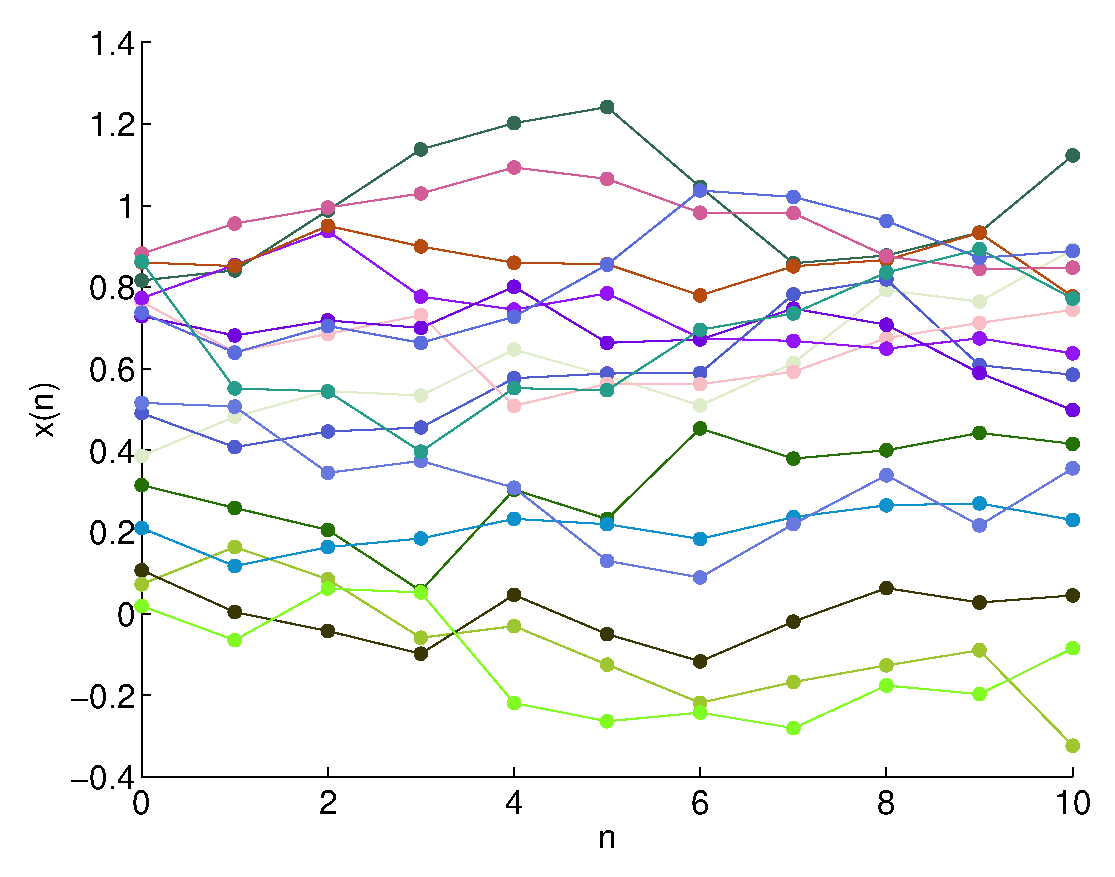
\includegraphics[width=\columnwidth]{./Figures/SignalRandomDisc.eps}
      \end{column}
    \end{columns}    
  \end{itemize}
  
  \rule{11cm}{0.04ex}
  \scriptsize
  
  $^1$ En principio, si la variable independiente es continua tendremos infinitas variables aleatorias, mientras que si la variable independiente es discreta tendremos tantas variables aleatorias como instantes de $n$ estemos analizando.
  
\end{frame}

\begin{frame}
  \frametitle{Estadísticos de las señales aleatorias}
  \vspace{-0.2cm}
  \footnotesize
  \begin{itemize}
    \item Se calculan de la misma forma que para conjuntos de variables aleatorias:
    \begin{itemize}
      \footnotesize
      \item Probabilidades:
      \begin{itemize}
        \scriptsize
        \item La probabilidad de la señal en cada instante: \\$p_{X(t)}(x(t))\triangleq \color{blue}p_X(x,t)$.
        \item La probabilidad conjunta de 1 señal en 2 instantes:\\$p_{X(t_1)X(t_2)}(x(t_1),x(t_2))\triangleq \color{blue}p_X(x_1,t_1,x_2,t_2)$.\\
        \item La probabilidad conjunta de 2 señales en 2 instantes:\\$p_{X_i(t_i)X_j(t_j)}(x_i(t_i),\!x_j(t_j))\!\triangleq \color{blue}\! p_{X_iX_j}(x_i,\!t_i,\!x_j,\!t_j)$.
      \end{itemize}

      \item Estadísticos habituales:

      \begin{itemize}
        \scriptsize
        \item Media:\\$\color{blue}\mu_{X(t)}=\int_{-\infty}^\infty xp(x,t)dx$\\
        % $\mu_X(t)\triangleq \mu_{X(t)}=\int_{-\infty}^\infty x(t)p(x(t))dx(t)=\int_{-\infty}^\infty xp(x,t)dx$
        \item Valor cuadrático medio:\\$\color{blue}\Psi_X(t)\triangleq \int_{-\infty}^\infty x^2p(x,t)dx$\\
        % $\Psi_X(t)\triangleq  E(X^2(t))=\int_{-\infty}^\infty x^2(t)p(x(t))dx(t)=\int_{-\infty}^\infty x^2p(x,t)dx$\\
        \item Correlación cruzada:\\$\color{blue}\phi_{X_i(t_i),X_j(t_j)} \triangleq\int_{-\infty}^\infty x_ix_jp(x_i,t_i,x_j,t_j)dx_idx_j$\\
        % $\phi_{X_i,X_j}(t_i,t_j) \triangleq \phi_{X_i(t_i),X_j(t_j)}=\int_{-\infty}^\infty x_i(t_i)x_j(t_j)p(x_i(t_i),x_j(t_j))dx_i(t_i)dx_j(t_j)=\int_{-\infty}^\infty x_ix_jp(x_i,t_i,x_j,t_j)dx_idx_j$
        \item Autocorrelación:\\$\color{blue}\phi_{X(t_1),X(t_2)}\triangleq\int_{-\infty}^\infty x_1x_2p(x_1,t_1,x_2,t_2)dx_1dx_2$
        % $\phi_{XX}(t_1,t_2) \triangleq \phi_{X(t_1),X(t_2)}=\int_{-\infty}^\infty x(t_1)x(t_2)p(x(t_1),x(t_2))dx(t_1)dx(t_2)=\int_{-\infty}^\infty x_1x_2p(x_1,t_1,x_2,t_2)dx_1dx_2$
      \end{itemize}
    \end{itemize}
  \end{itemize}


  \rule{11cm}{0.04ex}
  \scriptsize

  Estas probabilidades se podrían obtener marginalizando de las conjuntas de la secuencia de la señal o de las secuencias de las señales las variables que no están involucradas en la probabilidad final.
\end{frame}


%%%%%%%%%%%%%%%%%%%%%%%%%%%%%%%%%%%%%%%%%%%%%%%%%


\begin{frame}[fragile]
  \frametitle{Tipos de señales aleatorias I}
  \vspace{-0.2cm}
  \footnotesize
  \begin{itemize}
    \item \alert{Señal Markoviana Discreta de Orden I: }
    \begin{itemize}
      \footnotesize
      \item Probabilidad de $x[n]$ solo depende de $x[n-1]$: $\color{blue}p(x[n]|x[n-1])$
      \vspace{0.1cm}
      \item Esto permite factorizar convenientemente:\\
      {\scriptsize
      \vspace{0.1cm}
      $p(x(0),x(1),\cdots,x(n))=$
      \vspace{0.1cm}
      \hspace{0.3cm}$\color{gray}=p(x[0])p(x[1]|x[0])p(x[2]|x[0],x[1])\cdots p(x[n]|x[0],\cdots,x[n-1])=$
      \vspace{0.1cm}
      \hspace{0.3cm}$\color{gray}=p(x[0])p(x[1]|x[0])p(x[2]|x[1])\cdots p(x[n]|x[n-1])=$
      \vspace{0.1cm}
      \hspace{0.3cm}$=p(x[0])\prod_{i=1}^n p(x[n]|x[n-1])$
      }
    \end{itemize}
  \end{itemize}

  \color{olivegreen}Ejemplo: random walk gaussiano\\
  \vspace{0.1cm}
  \color{gray}
  {\scriptsize
  $x[n] = x[n-1] + u[n-1]$\\[0.5ex]
  \hspace{0.8cm}$p(u[n])=\mathcal{N}_{\mu=0,\sigma^2=0.25}(u[n])$\\[0.5ex]
  \hspace{0.8cm}$p(x(0))=\mathcal{N}_{\mu=0,\sigma^2=1}(x(0))$\\[0.5ex]
  $p(x[n]|x[n-1])=\mathcal{N}(\mu=x[n-1],\sigma^2=0.25)$
  }
  \vspace{-0.5cm}
  \begin{columns}[c]
    \begin{column}{6.2cm}
      {\begin{lstlisting}[style=Matlab-editor,basicstyle=\scriptsize]
N = 100;
M = 1000;
x = zeros(N, M);
v = sqrt(0.25)*randn(N, M);
x(1, :) = randn(1, M);
for k = 2:N
  x(k, :) = x(k-1, :) + v(k-1, :);
end
      \end{lstlisting}}
    \end{column}
    \begin{column}{3.8cm}
      \vspace{0.2cm}
      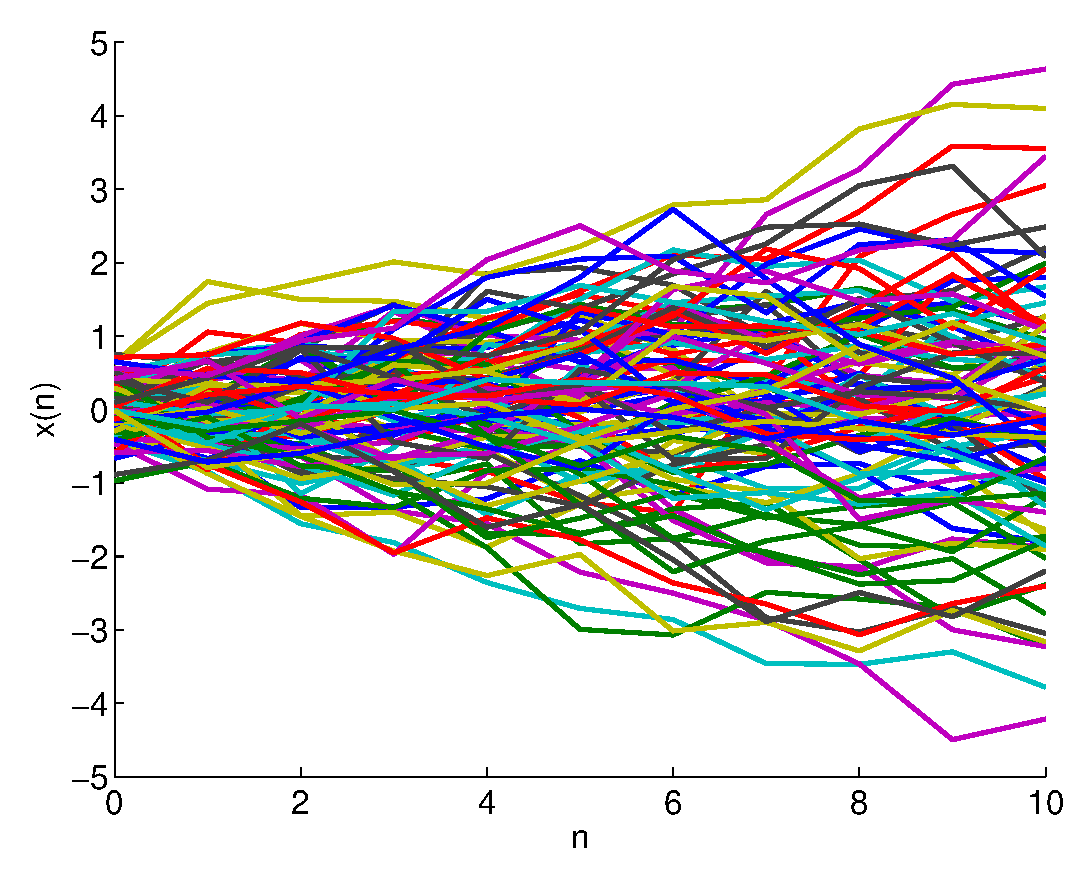
\includegraphics[width=\columnwidth]{./Figures/RandomWalk.eps}
    \end{column}
  \end{columns}

\end{frame}

%%%%%%%%%%%%%%%%%%%%%%%%%%%%%%%%%%%%%%%%%%%%%%

\begin{frame}
  \frametitle{Tipos de señales aleatorias II}
  \footnotesize

  \begin{itemize}
    \item \alert{Señal Markoviana Continua de Orden I: }
    \begin{itemize}
      \footnotesize
      \item Mientras que a la hora de modelar sistemas/señales discretos se utilizan los retardos para relacionar las variables, a la hora de modelar sistemas/señales continuos se utilizan las derivadas:
      \vspace{0.1cm}
      {\\\color{olivegreen}
      \hspace{0.5cm}Ejemplo discreto: $y(k)+y(k-1)+y(k-2)=x(k)$
      \vspace{0.1cm}
      \\
      \hspace{0.5cm}Ejemplo continuo: $\ddot y(t)+ \dot y(t) +y(t)=x(t)$
      \vspace{0.1cm}
      \color{black}}
      \item Por lo tanto, la relación probabilística que se establece en señales Markovianas discretas entre una señal y su versión retardada, en señales Markovianas continuas se establece entre la derivada de la señal y la señal sin derivar:
        $p(\dot x(t)|x(t))$

      \vspace{0.1cm}
      \hspace{0.5cm}\color{olivegreen}Ejemplo: proceso Markov gaussiano \color{gray}\\
      \vspace{0.1cm}
      \hspace{1.0cm}$\dot x(t)\!=\!x(t)\!+\!u(t)$ con:\\
      \scriptsize
      \vspace{0.1cm}
      \hspace{1.5cm}$p(u(t))=\mathcal{N}_{\mu=0,\sigma=1}(x(t);0.25)$\\
      \vspace{0.1cm}
      \hspace{1.5cm}$p(x(0)))=\delta(x(0))$\\
      \vspace{0.2cm}
      \hspace{0.8cm}$p(\dot x(t)|x(t))\!=\!\mathcal{N}_{\mu=x(t),\sigma^2=0.25}(\dot x(t))$
    \end{itemize}
  \end{itemize}

\end{frame}

%%%%%%%%%%%%%%%%%%%%%%%%%%%%%%%%%%%%%%%%%%%%%%

\begin{frame}
\frametitle{Tipos de señales aleatorias III}
  \vspace{-0.2cm}
  \footnotesize

  \begin{itemize}
    \item \alert{Señales aleatorias estacionarias (en sentido amplio): }
    \begin{itemize}
      \footnotesize
      \item La función de probabilidad no depende del tiempo: $\color{blue}p(x(t_1))=p(x(t_2))\triangleq p(x)$
      \vspace{0.1cm}
      \item Los estadísticos de una variable no dependen del tiempo:
      \begin{itemize}
        \scriptsize
        \item Media: \\$\color{blue}\mu_X(t)=\color{gray}\int_{-\infty}^\infty x(t)p(x(t))dx(t)=\int_{-\infty}^\infty xp(x)dx= \alert{\mu_X}$
        \item Valor cuadrático medio: \\$\color{blue}\Psi_X(t)=\color{gray}\int_{-\infty}^\infty x^2(t)p(x(t))dx(t)=\int_{-\infty}^\infty x^2p(x)dx=\alert{\Psi_X}$
        \item Varianza: \\$\color{blue}\sigma^2_X(t)=\color{gray}\Psi_X(t)-\mu^2_X(t)=\Psi_X-\mu^2_X=\alert{\sigma^2_X}$
      \end{itemize}
      \item Los estadísticos de dos variables dependen de la diferencia temporal:
      \begin{itemize}
        \scriptsize
        \item Correlación cruzada: $\color{blue}\phi_{X_i,X_j}(t_i,t_j) =\color{gray}\int_{-\infty}^\infty x_i(t_i)x_j(t_j)p(x_i(t_i),x_j(t_j))dx_i(t_i)dx_j(t_j)=$
        $\color{gray}\int_{-\infty}^\infty x_i(t)x_j(t+\tau)p(x_i(t),x_j(t+\tau))dx_i(t)dx_j(t+\tau)=\alert{\phi_{X_iX_j}(\tau)}$
        \item Autocorrelación:
        $\color{blue}\phi_{XX}(t_1,t_2)=\color{gray}\int_{-\infty}^\infty x(t_1)x(t_2)p(x(t_1),x(t_2))dx(t_1)dx(t_2)=$
        $\color{gray}\int_{-\infty}^\infty x(t)x(t+\tau)p(x(t),x(t+\tau))dx(t)dx(t+\tau)=\alert{\phi_{XX}(\tau)}$
      \end{itemize}
    \end{itemize}
  \end{itemize}
\end{frame}

%%%%%%%%%%%%%%%%%%%
\begin{frame}
  \frametitle{Tipos de señales aleatorias IV}
\footnotesize

\vspace{-0.1cm}

\color{olivegreen}¿Cuales de las señales siguientes son estacionarias (en sentido amplio)?





%%%%%%%%%%%%%%%%%%%%%%%%

\begin{columns}[T]
\hspace{-0.5cm}\begin{column}{7cm}

\color{olivegreen}Ej1: ¿sistema discreto con variables $x(n)$ independientes y $p(x(n))=\mathcal{U}_{[a,b]}(x(n))$


 \color{gray}


\visible<2->{
\vspace{0.0cm}

Si, ya que las variables son independientes y tienen la misma función de probabilidad a lo largo del tiempo.
}
\end{column}
\begin{column}{2.5cm}
\visible<2->{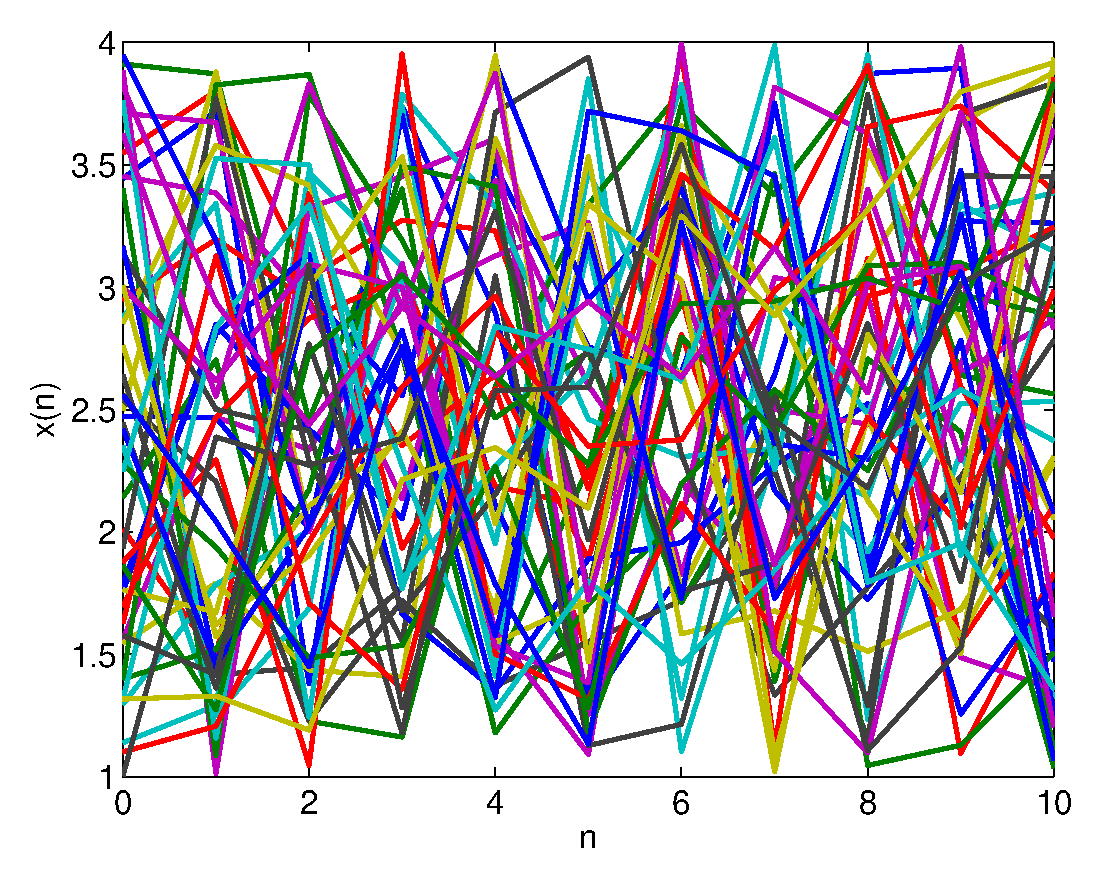
\includegraphics[width=2cm]{./Figures/Est1.eps}}
\end{column}
\end{columns}



%%%%%%%%%%%%%%%%%%%%%%%%%

\vspace{0.2cm}

\visible<3->{
\begin{columns}[T]
\hspace{-0.5cm}\begin{column}{7cm}




\color{olivegreen}Ej2: ¿sistema discreto con variables $x(n)$ independientes y $p(x(n))=\mathcal{N}_X(x(n);\mu_x,(0.5)^{n})$


 \color{gray}


\visible<4->{
\vspace{0.1cm}

No, ya que aunque las variables son independientes la función de probabilidad cambia a lo largo del tiempo.
}
\end{column}
\begin{column}{2.5cm}
\visible<4->{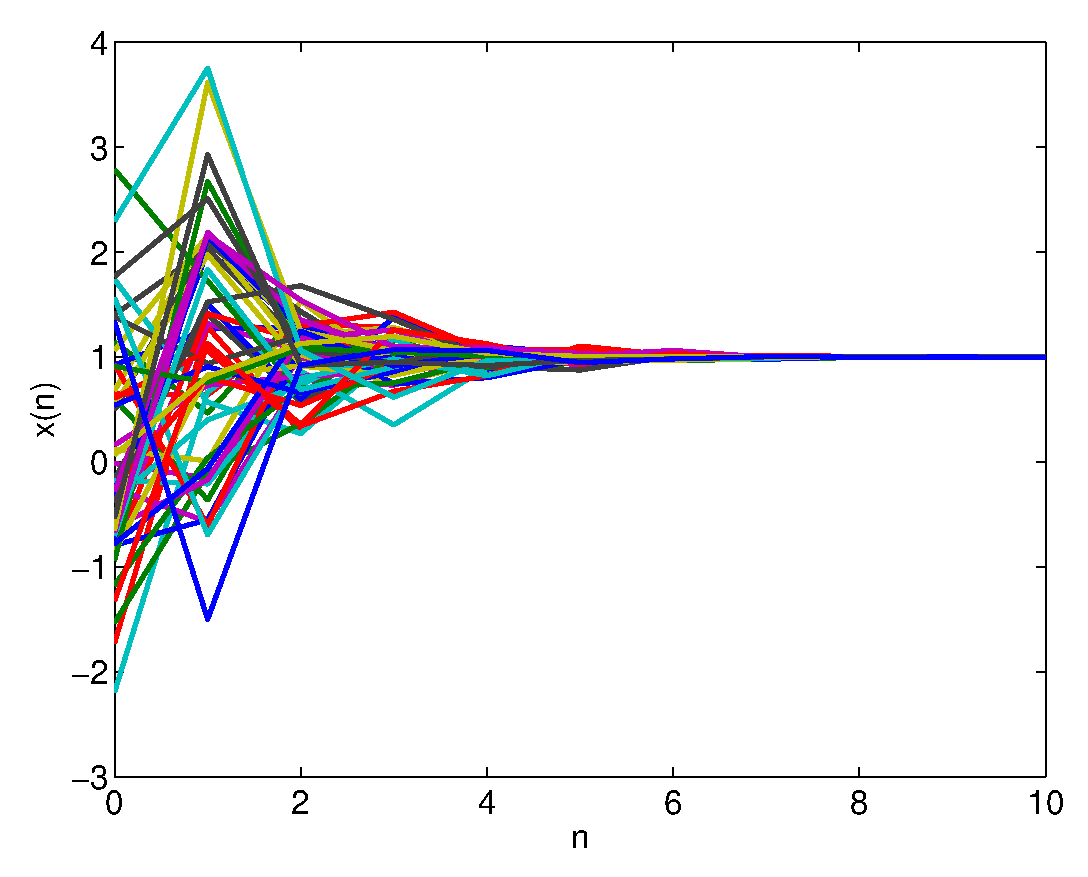
\includegraphics[width=2cm]{./Figures/Est2.eps} }
\end{column}
\end{columns}
}

%%%%%%%%%%%%%%%%%%%%%%%%%%%%%%%%%


\vspace{0.3cm}

\visible<5->{
\begin{columns}[T]
\hspace{-0.5cm}\begin{column}{7cm}

\color{olivegreen}Ej3: ¿random walk gaussiano discreto propuesto? \color{gray}

\visible<6->{
No, ya que la varianza del proceso (estadístico de una variable) aumenta a lo largo del tiempo.
}
\end{column}
\begin{column}{2.5cm}
\visible<5->{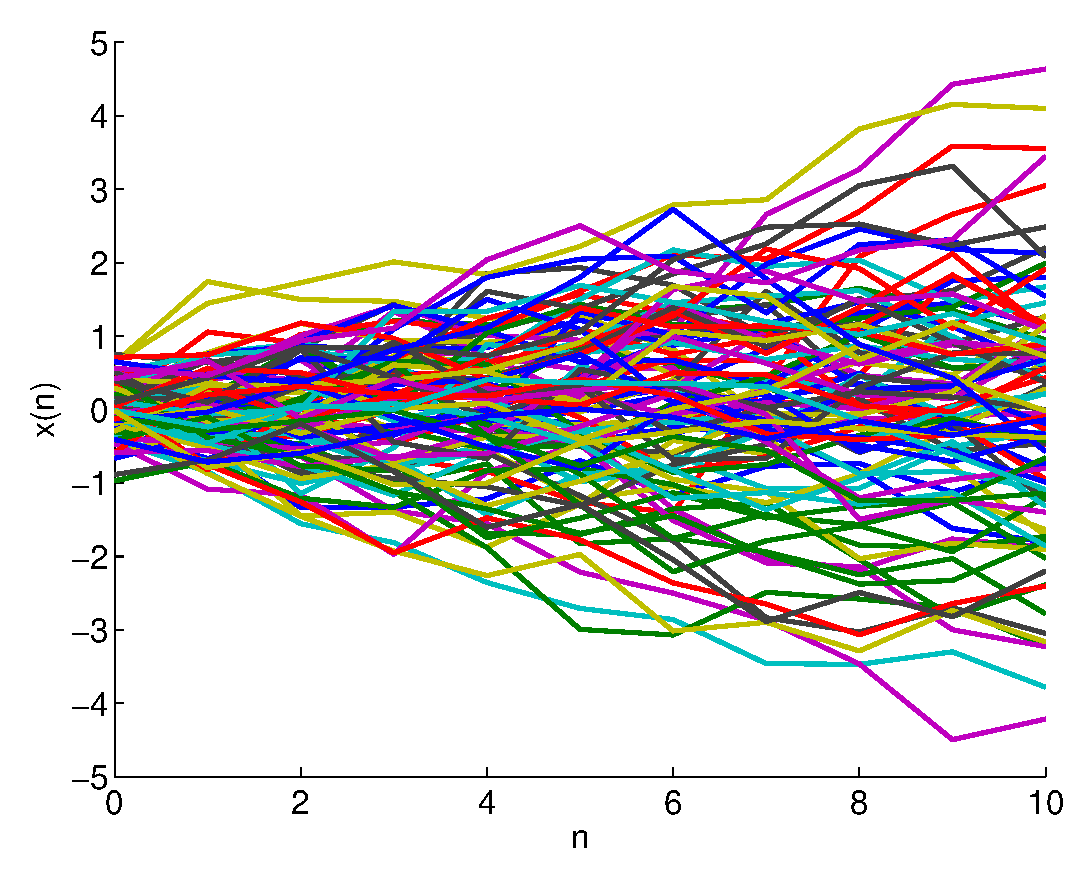
\includegraphics[width=2cm]{./Figures/RandomWalk.eps}}
\end{column}
\end{columns}

}

\vspace{0.1cm}

\visible<7->{
\begin{columns}[T]
\hspace{-0.5cm}\begin{column}{7cm}

\color{olivegreen}Ej4: Markoviano discreto $p(x(0))=U_{[a,b]}(x(0))$ y $p(x(n)|x(n-1))=\delta(x(n)-x(n-1))$  \color{gray}


\visible<8->{
\vspace{0.0cm}

Si, ya que se puede demostrar que $p(x(n))=U_{[a,b]}(x(n))$.
}
\end{column}
\begin{column}{2.5cm}
\visible<6->{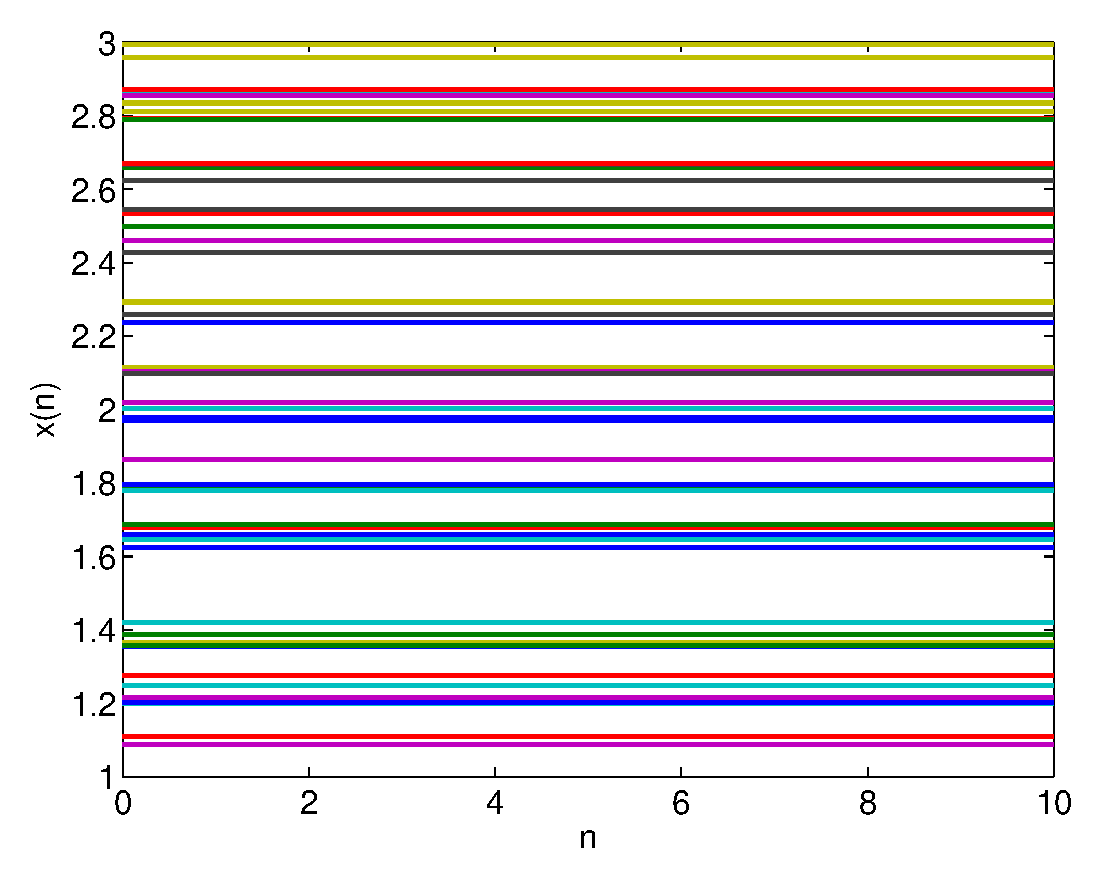
\includegraphics[width=2cm]{./Figures/Est3.eps}}
\end{column}
\end{columns}

}


\end{frame}

%%%%%%%%%%%%%%%%%%%%%%%%%%%%%%%%%%%%%%%%%%
\begin{frame}
  \frametitle{Tipos de señales aleatorias V}
    \vspace{-0.2cm}
    \footnotesize
    \begin{itemize}
      \item \alert{Señales ergódicas: }
      \begin{itemize}
        \footnotesize
        \item Son señales aleatorias \alert{estacionarias}.
        \item Una muestra (secuencia de valores) es representativa de la señal.
        \vspace{0.1cm}
        \item Los estadísticos se caracterizan directamente a partir de una muestra:
        \begin{itemize}\scriptsize
          \item $\mu_X \triangleq \lim_{T \rightarrow \infty} \frac{1}{2T}\int_{-T}^T x(t)dt$
          \item $\Psi_X \triangleq \lim_{T \rightarrow \infty} \frac{1}{2T} \int_{-T}^T x^2(t)dt$
          \item $\phi_{X_i,X_j}(\tau)  \triangleq \lim_{T \rightarrow \infty} \frac{1}{2T}\int_{-T}^T x_i(t)x_j(t+\tau)dt$
          \item $\phi_{XX}(\tau) \triangleq \lim_{T \rightarrow \infty} \frac{1}{2T}\int_{-T}^T x(t)x(t+\tau)dt$
        \end{itemize}
    \end{itemize}
  \end{itemize}
\end{frame}


\begin{frame}
\frametitle{Tipos de señales aleatorias VI}

\footnotesize

\vspace{-0.1cm}

\color{olivegreen}¿Cuales de las señales siguientes son ergódicas?





%%%%%%%%%%%%%%%%%%%%%%%%

\begin{columns}[T]
\hspace{-0.5cm}\begin{column}{7cm}

\color{olivegreen}Ej1: ¿sistema discreto con variables $x(n)$ independientes y $p(x(n))=\mathcal{U}_{[a,b]}(x(n))$


 \color{gray}


\visible<2->{
\vspace{0.0cm}

Si, ya que es estacionario y se puede obtener los estadísticos de una única secuencia de valores.
}
\end{column}
\begin{column}{2.5cm}
\visible<2->{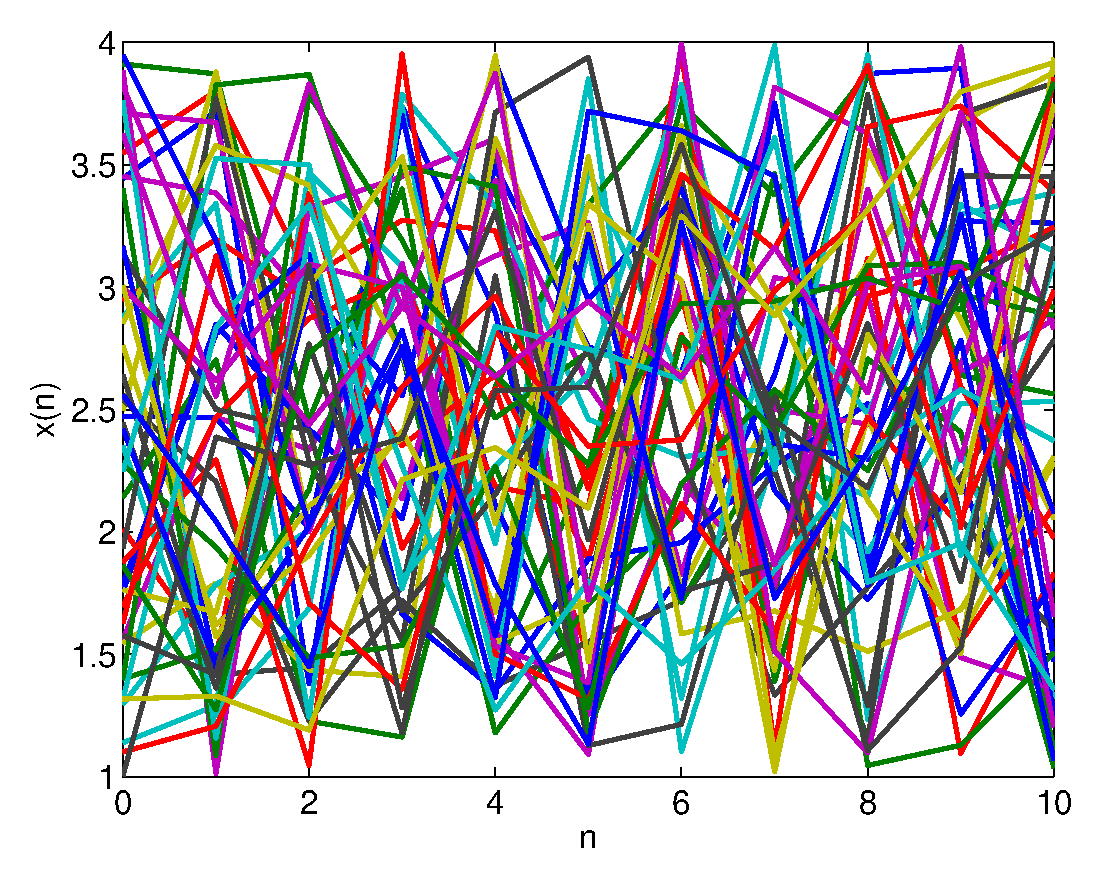
\includegraphics[width=2cm]{./Figures/Est1.eps}}
\end{column}
\end{columns}



%%%%%%%%%%%%%%%%%%%%%%%%%

\vspace{0.2cm}

\visible<3->{
\begin{columns}[T]
\hspace{-0.5cm}\begin{column}{7cm}




\color{olivegreen}Ej2: ¿sistema discreto con variables $x(n)$ independientes y $p(x(n))=\mathcal{N}_X(x(n);\mu_x,(0.5)^{n})$


 \color{gray}


\visible<4->{
\vspace{0.1cm}

No, ya que no es estacionario.
}
\end{column}
\begin{column}{2.5cm}
\visible<4->{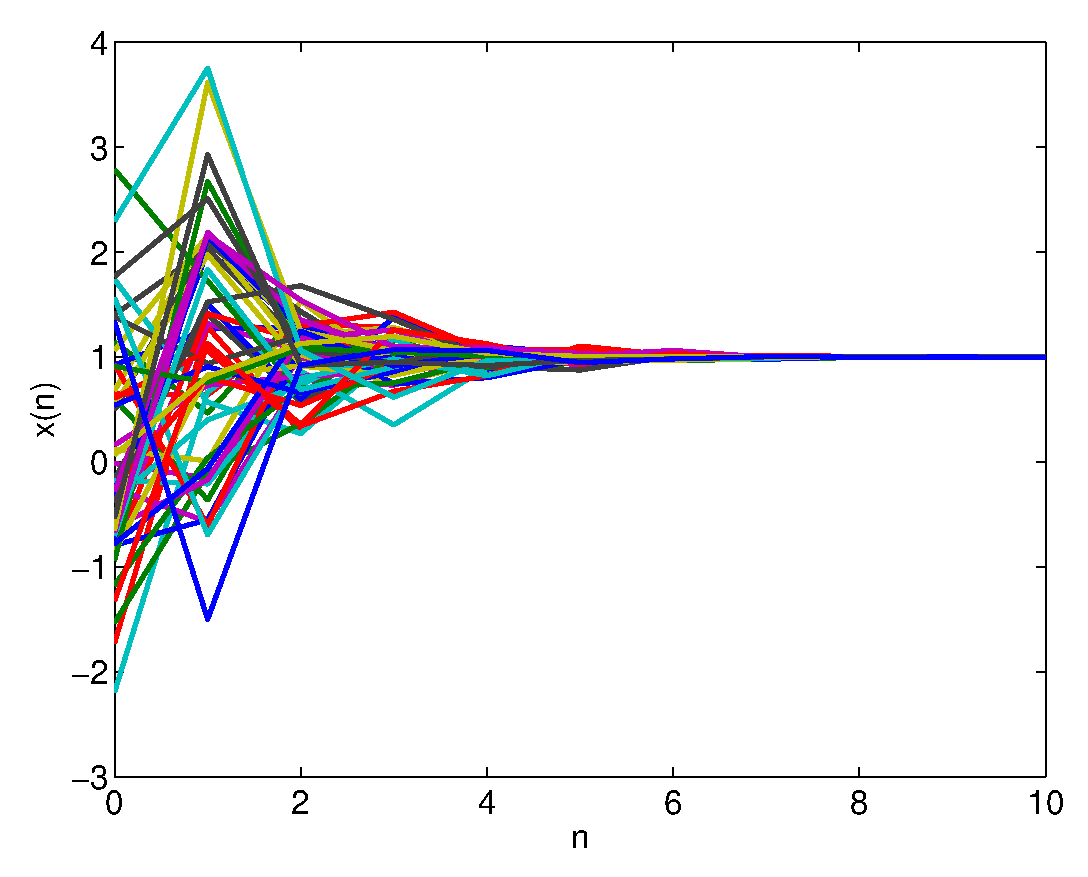
\includegraphics[width=2cm]{./Figures/Est2.eps} }
\end{column}
\end{columns}
}

%%%%%%%%%%%%%%%%%%%%%%%%%%%%%%%%%


\vspace{0.3cm}

\visible<5->{
\begin{columns}[T]
\hspace{-0.5cm}\begin{column}{7cm}

\color{olivegreen}Ej3: ¿random walk gaussiano discreto propuesto? \color{gray}


\visible<6->{
\vspace{0.1cm}
No, ya que no es estacionario.
}
\end{column}
\begin{column}{2.5cm}
\visible<5->{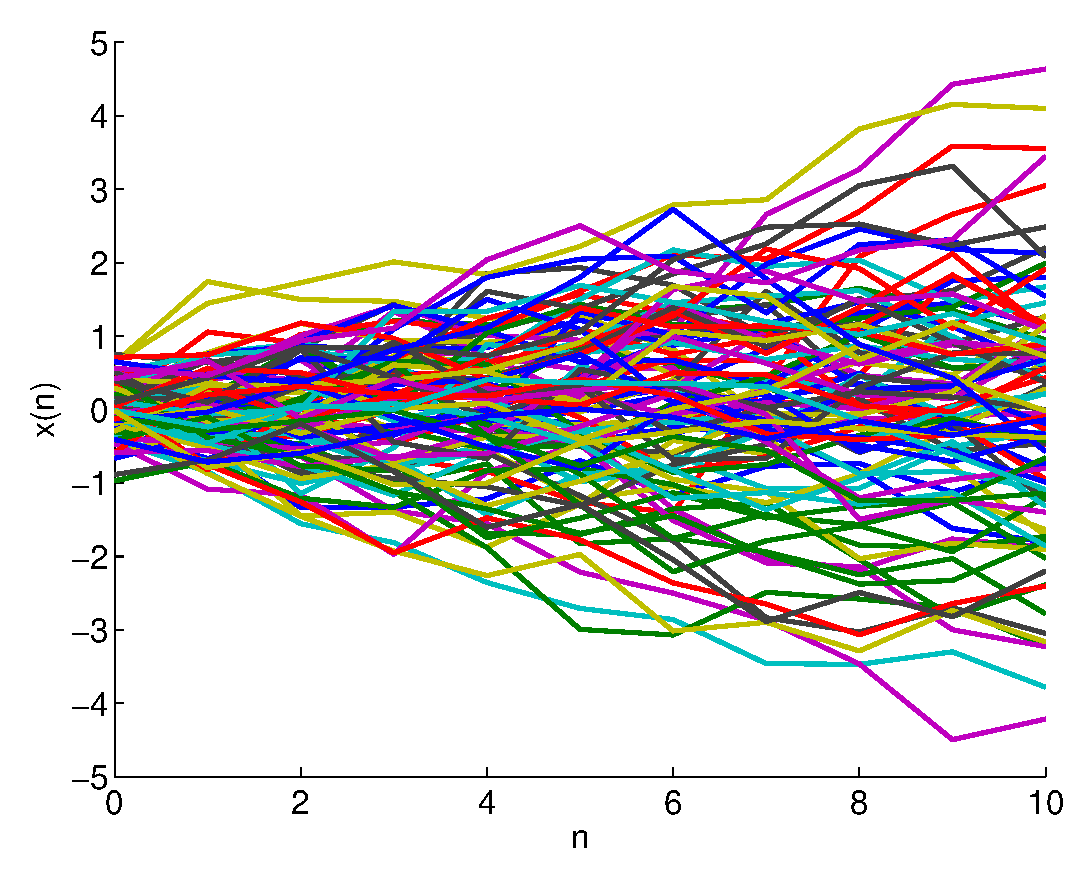
\includegraphics[width=2cm]{./Figures/RandomWalk.eps}}
\end{column}
\end{columns}

}

\vspace{0.1cm}

\visible<7->{
\begin{columns}[T]
\hspace{-0.5cm}\begin{column}{7cm}

\color{olivegreen}Ej4: Markoviano discreto $p(x(0))=U_{[a,b]}(x(0))$ y $p(x(n)|x(n-1))=\delta(x(n)-x(n-1))$  \color{gray}


\visible<8->{
\vspace{0.0cm}

No, ya que una secuencia de valores no es representativa de la muestra (cada señal toma un valor constante).
}
\end{column}
\begin{column}{2.5cm}
\visible<6->{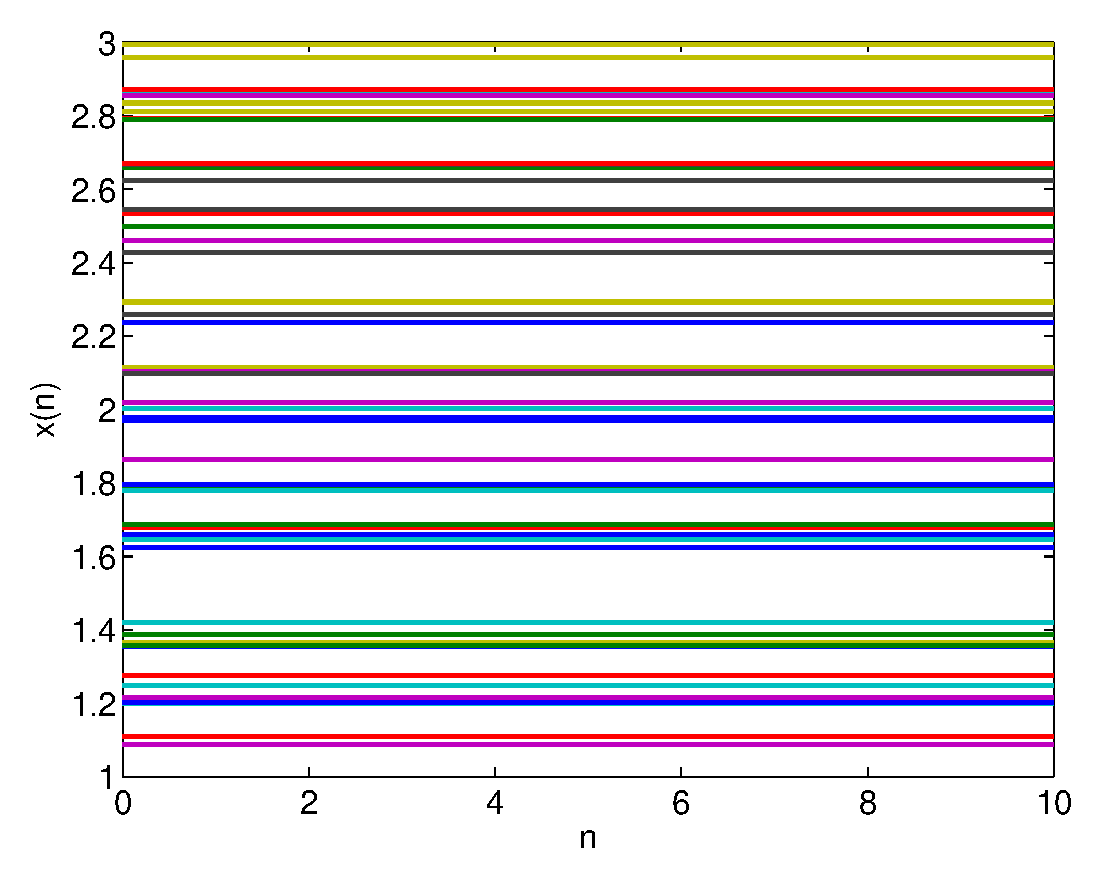
\includegraphics[width=2cm]{./Figures/Est3.eps}}
\end{column}
\end{columns}

}

\end{frame}





%%%%%%%%%%%%%%%%%%%%%%
\begin{frame}
  \frametitle{Señales aleatorias estacionarias: Propiedades I}
  \footnotesize

  \begin{itemize}
    \item $\mu_X$, $\Psi_X$, y $\sigma_X^2$ son constantes en el tiempo.
    \item $\phi_{XY}(\tau)$, $\phi_{XX}(\tau)$, y $\phi_{XY}(\tau)$ dependen sólo de la diferencia temporal $\tau$.
    \item Relaciones con la autocorrelación:
    \begin{itemize}
      \footnotesize
      \item $\phi_{XX}(0)=\Psi_X=E(X^2)$.\\
      {\scriptsize\color{gray}%\vspace{0.1cm}
      $\Psi_X=E(X^2)=\int x^2(t) p(x(t))dx(t)$\\
      $\phi_{XX}(\tau)=\int x(t)x(t+\tau) p(x(t),x(t+\tau))dx(t)$
      }
      \item $\phi_{XX}(\infty)=|\mu_X|^2.$
      \item $\phi_{XX}(0)>\phi_{XX}(\tau)$  (el máximo de la autocorrelación está en cero)
    \end{itemize}
  \end{itemize}
  \begin{alertblock}{¿Como sabemos si una señal tiene o no componente determinista?}
    \begin{itemize}
      \item Si la señal es aleatoria, $\phi_{XX}(\tau)\rightarrow|\mu_X|^2$ para $t>>0$.
      \item Si tiene componente determinista, $\phi_{XX}(\tau)$ no tiende a $|\mu_X|^2$.
      \item Si la parte determinista es periódica, $\phi_{XX}(\tau)$ también lo mostrará.
    \end{itemize}
\end{alertblock}
\end{frame}

%%%%%%%%%%%%%%%%%%%%%%%%%%%%%%%%%%%%%%%%%%%%%%%

\begin{frame}[fragile]
  \frametitle{Señales aleatorias estacionarias: Propiedades II}
  \footnotesize
  \vspace{-0.1cm}
  \color{olivegreen}Ejemplos de autocorrelación de señales ergódicas (usadas como casos de estacionarias porque permiten cálculos a partir de una secuencia de valores).

  \begin{itemize}
    \scriptsize
    \item \color{blue}\texttt{[phixy,lags]=xcorr(x,y,limk,'unbiased')}: \color{black}cálculo de la correlación$^1$ cruzada de las señales x e y.
    \item \color{blue}\texttt{[phixy,lags]=xcorr(x,limk,'unbiased')}: \color{black} cálculo de la autocorrelación$^1$ de la señal x.
  \end{itemize}
  \color{olivegreen}Ej1: Sistema continuo con variables $x(t)$ independientes y $p(x(t))=\mathcal{N}(x(t);5,1)$\color{black}\\
  \begin{columns}[T]
    \hspace{-0.5cm}\begin{column}{6.75cm}
      \vspace{0.1cm}
      Lo discretizamos con periodo $T_s=0.01$\\
    {\begin{lstlisting}[style=Matlab-editor,basicstyle=\scriptsize]
Ts = 0.01;
t = 0:Ts:10;
x = 5 + randn(size(t));
[xc, lags] = xcorr(x, 100, 'unbias');
      \end{lstlisting}}
    \end{column}
    \begin{column}{4cm}
      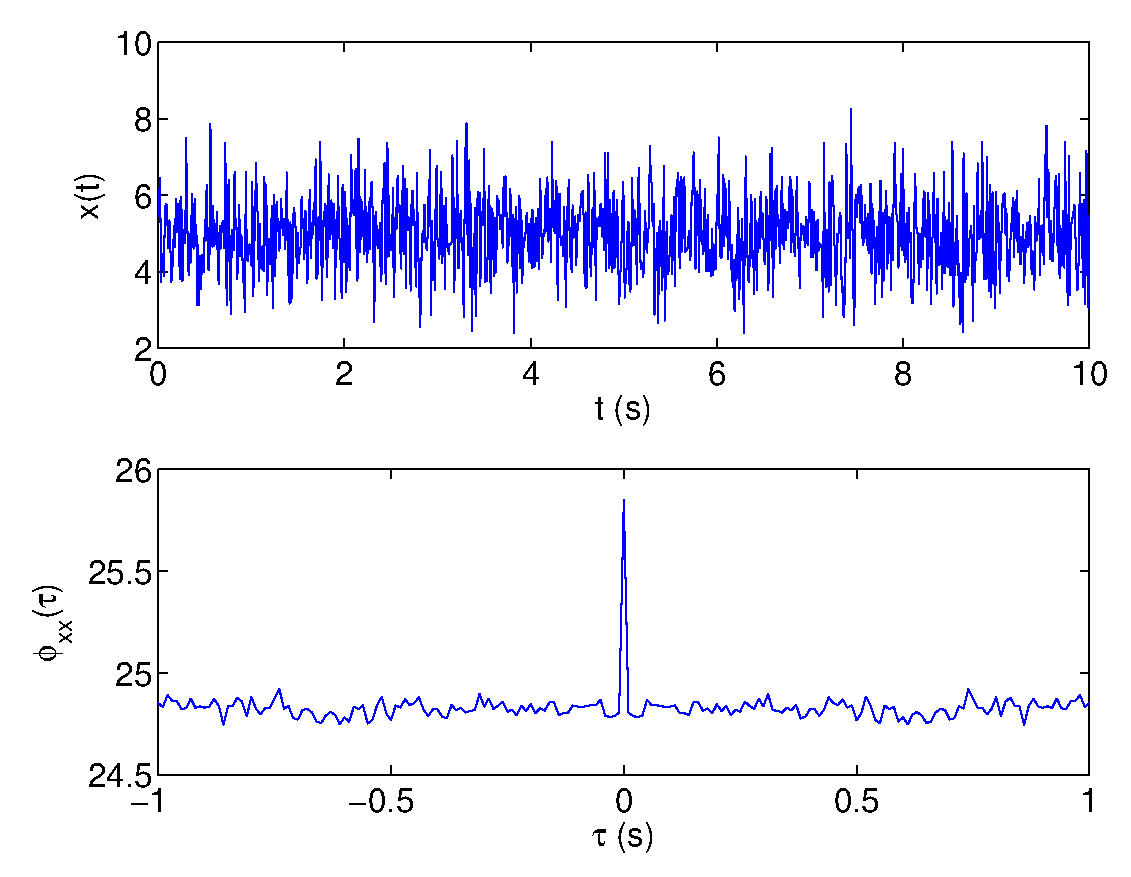
\includegraphics[width=3.2cm]{./Figures/Auto1.eps}
      \scriptsize
      \color{gray}
      $\phi_{XX}(0)=\Psi_X=\sigma^2_X+\mu^2_X=26$

      $\phi_{XX}(\infty) \rightarrow \mu^2_X=25$
    \end{column}
  \end{columns}

  \rule{11cm}{0.04ex}
  \scriptsize

  $^1$\color{blue}\texttt{limk} \color{black} se utiliza para limitar los valores de la $k$ sobre los que se calcula la correlación y la autocorrelación. Los límites temporales están $\tau=\pm T_s limk$.

\end{frame}

%%%%%%%%%%%%%%%%%%%%%%%%%

\begin{frame}[fragile]
  \frametitle{Señales aleatorias estacionarias: Propiedades III}
  \footnotesize
  \color{olivegreen}Ej2: Sistema continuo con variables $x(t)$ independientes y $p(x(t))=\mathcal{U}_{[2,6]}(x(t))$\color{black}
  \vspace{0.5cm}
  \begin{columns}[T]
    \hspace{-0.5cm}\begin{column}{6.75cm}
    Lo discretizamos con periodo $T_s=0.01$\\
    {\begin{lstlisting}[style=Matlab-editor,basicstyle=\scriptsize]
Ts = 0.01;
t = 0:Ts:10;
x = 2 + 4*rand(size(t));
[xc, lags] = xcorr(x, 100, 'unbias');

figure();
subplot(2,1,1);
  plot(t,x);
  xlabel('t (s)');
  ylabel('x(t)');
subplot(2,1,2);
  plot(lags*Ts,xc);
  xlabel('\tau (s)');
  ylabel('\phi_{xx}(\tau)');
    \end{lstlisting}}

    \end{column}
    \begin{column}{4cm}
      \vspace{0.5cm}
      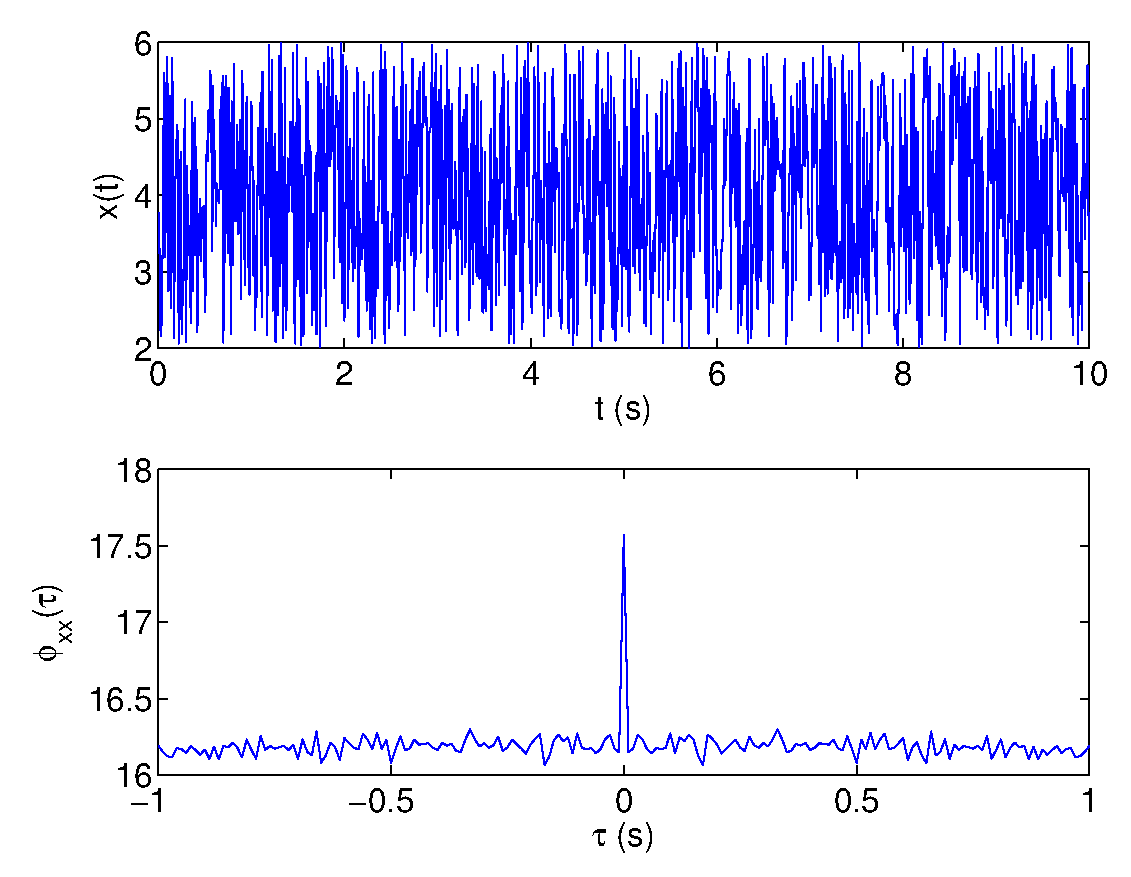
\includegraphics[width=\columnwidth]{./Figures/Auto2.eps}
      \scriptsize
      \color{gray}\\
      $\phi_{XX}(0)\!=\!\Psi_X\!=\!\frac{b^2+a^2+ab}{3}\!=\!17.3$\\
      $\phi_{XX}(\infty) \rightarrow \mu^2_X=\left(\frac{b+a}{2}\right )^2=16$
    \end{column}
  \end{columns}


\end{frame}


\begin{frame}[fragile]
  \frametitle{Señales aleatorias estacionarias: Propiedades III}
  \footnotesize
  \color{olivegreen}Ej3: Sistema continuo determinista con $x(t)=sen(2\pi F t)$ con $F=10$ Hz.\\
  \begin{columns}[c]
    \hspace{-0.5cm}\begin{column}{6.5cm}
    \color{black}\\
    \vspace{0.2cm}
    Lo discretizamos con periodo $T_s=0.01$
    % \vspace{-0.3cm}
    {\begin{lstlisting}[style=Matlab-editor,basicstyle=\scriptsize]
Ts = 0.01;
t=0:Ts:10;
x = sin(2*pi*F*t);
[xc, lags] = xcorr(x,100,'unbias');

figure();
subplot(2,1,1);
  plot(t,x);
  xlabel('t (s)');
  ylabel('x(t)');
subplot(2,1,2);
  plot(lags*Ts,xc);
  xlabel('\tau (s)');
  ylabel('\phi_{xx}(\tau)');    
    \end{lstlisting}}
    \end{column}
    \begin{column}{4cm}
      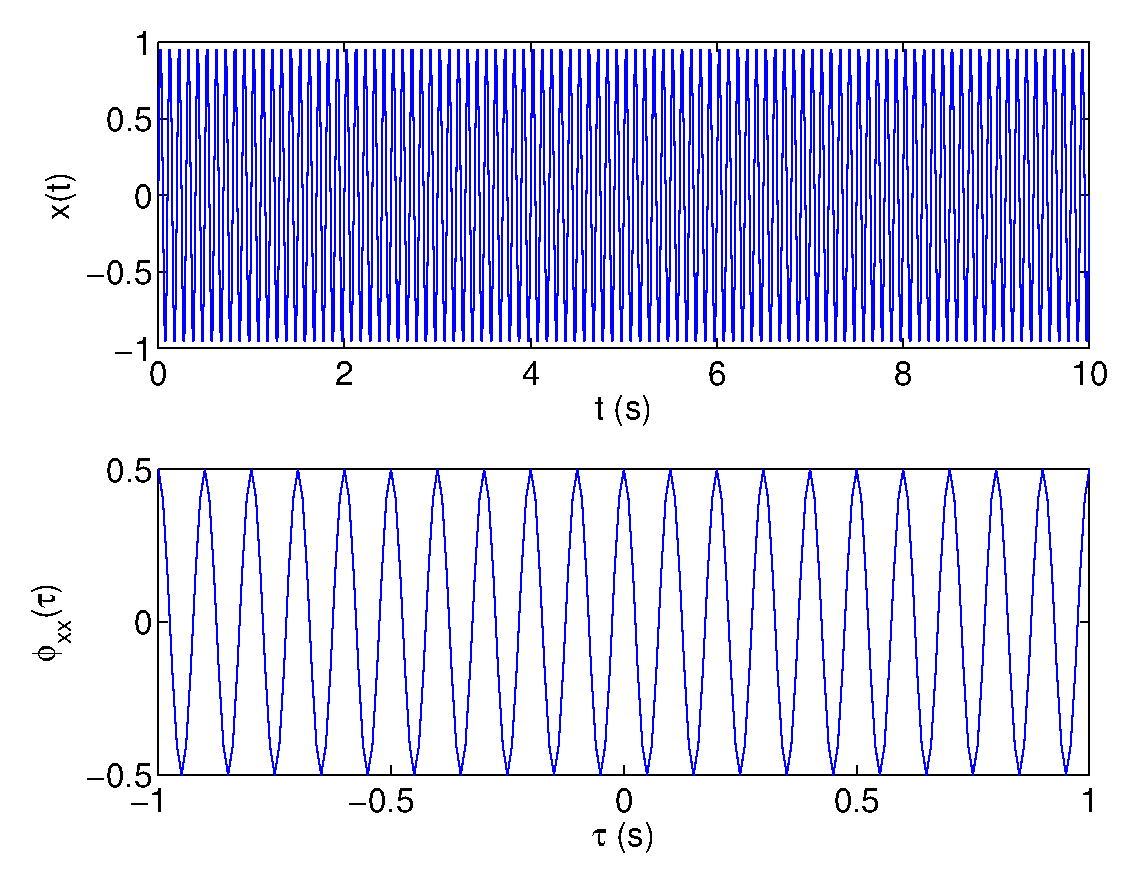
\includegraphics[width=4cm]{./Figures/Auto3.eps}
    \end{column}
  \end{columns}

\end{frame}

\begin{frame}
  \frametitle{Señales aleatorias estacionarias: Propiedades IV}
  \footnotesize
    \begin{itemize}
    \item Correlación cruzada:
    \begin{itemize}
      \footnotesize
      \item No tiene necesariamente un máximo en $\tau=0$
      \vspace{0.1cm}
      \item $\phi_{XY}(\tau)=\phi_{YX}(-\tau)$
      \vspace{0.1cm}
      \item  $|\phi_{XY}(\tau)|^2 \le \phi_{XX}(0) \phi_{YY}(0)$
      \vspace{0.1cm}
      \item  $|\phi_{XY}(\tau)| \le \frac{1}{2} [\phi_{XX}(0) +\phi_{YY}(0)]$
      \vspace{0.1cm}
      \item  Si las variables son independientes $\phi_{XY}(0)=\mu_X \mu_Y$.
    \end{itemize}
    \item Algunas aplicaciones de la correlación cruzada:
    \begin{itemize}
      \footnotesize
      \item Determinar retardos entre señales. 
      \item Determinación de caminos de transmisión con diferentes retardos.
      \item Recuperar señales con ruido 
    \end{itemize}
  \end{itemize}
\end{frame}

\begin{frame}
  \frametitle{Señales aleatorias estacionarias: Propiedades V}
  \footnotesize
  \color{olivegreen}Ejemplos de aplicación de correlación cruzada de señales.
  \vspace{0.2cm}

  \begin{columns}[T]
  \hspace{-0.3cm}\begin{column}{7.25cm}
    \color{olivegreen}Ej1: Calcular el desfase de las señales $x(t)=sinc(t-2)$ y $y(t)=sinc(t-3)$
    \color{black}
    \vspace{0.1cm}\\
    Lo discretizamos con periodo $T_s=0.01$
    \vspace{-0.4cm}
    \lstinputlisting{./Matlab/Corr1.m}
    \end{column}
    \begin{column}{4cm}
      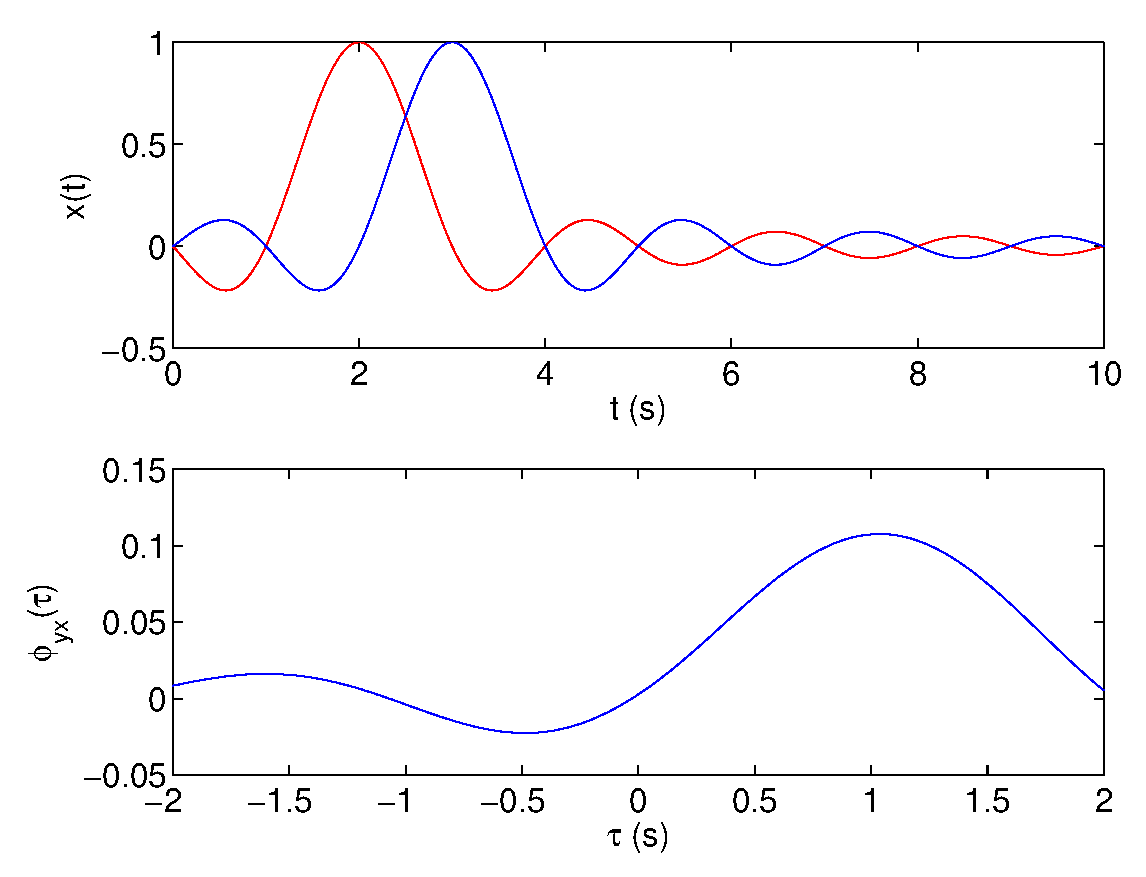
\includegraphics[width=3.2cm]{./Figures/CrossCorr1.eps}
      \scriptsize
      \color{gray}
      Máximo en $\tau=1$, tiempo que está retardada la señal.
    \end{column}
  \end{columns}
  \vspace{0.2cm}

  \begin{columns}[T]
  \hspace{-0.35cm}\begin{column}{7.25cm}
    \color{olivegreen}Ej2: Localizar la señal $x(t)=sinc(t-2)$ en $y(t)=sinc(t-3)+u(t)$ con $u(t)\sim \mathcal{N}_U(u,0,4)$
    \color{black}\\
    \vspace{0.1cm}
    Lo discretizamos con periodo $T_s=0.01$
    \vspace{-0.4cm}
    \lstinputlisting{./Matlab/Corr2.m}
    \end{column}
    \begin{column}{4cm}
      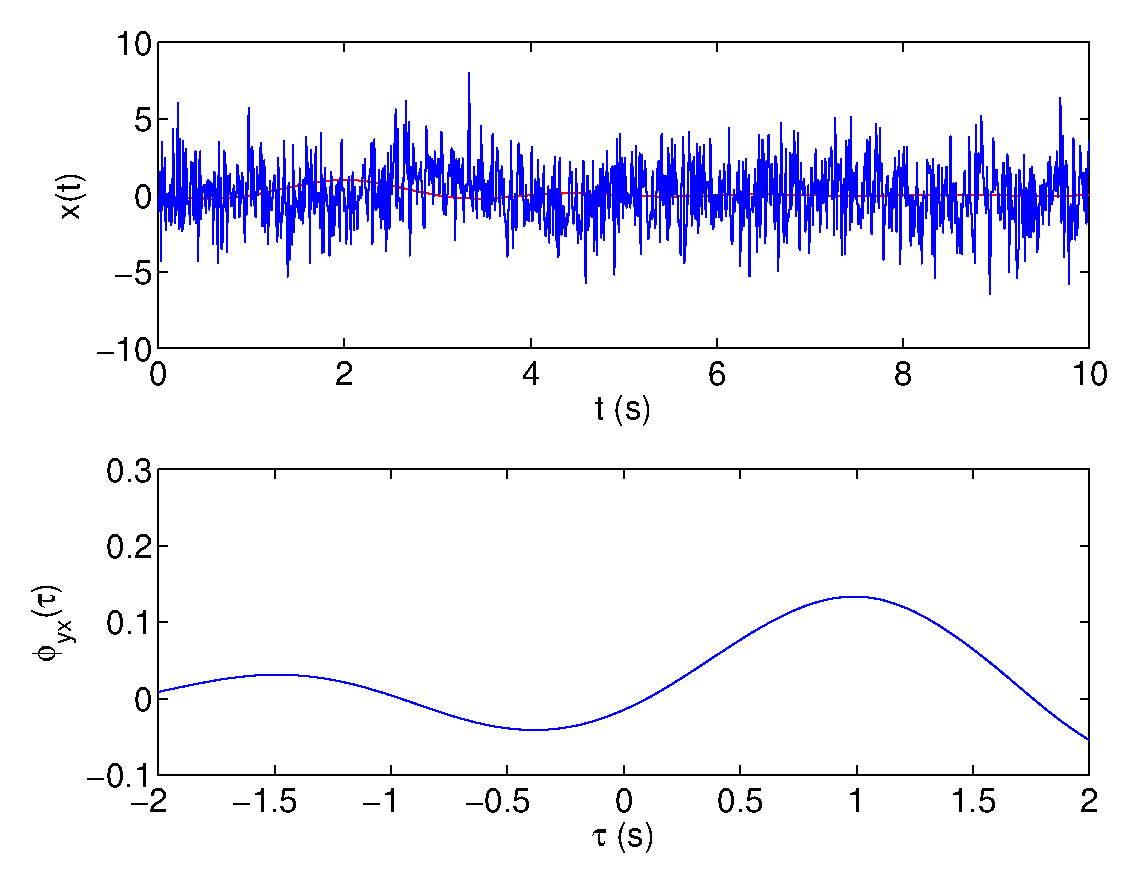
\includegraphics[width=3.2cm]{./Figures/CrossCorr2.eps}
      \scriptsize
      \color{gray}
      Máximo en $\tau=1$,  tiempo que está retardada la señal determinista buscada
    \end{column}
  \end{columns}
\end{frame}




\begin{frame}
  \frametitle{Potencia de una señal aleatoria}
    \vspace{-0.2cm}
    \footnotesize
    \begin{itemize}
    \item La potencia de una señal aleatoria$^1$ se define como $E\{P(x[n])\}$:
    
    $P_X=E\{\lim_{N \rightarrow \infty } \frac{1}{2N+1}\sum_{n=-N}^{N} x^2[n]\}=\lim_{N \rightarrow \infty } \frac{1}{2N+1} \sum_{n=-N}^{N} E\{x^2[n]\}$
    
    \item Si $x[n]$ es una señal aleatoria estacionaria se cumple que:
    
    \begin{itemize}
      \footnotesize
      \item $P_X=E\{x^2[n]\}$.
      \item $P_X=\phi_{XX}(0)=\sigma^2_X+\mu_x^2$.
    \end{itemize}
    
  
    \item Por lo tanto, en el caso de las señales aleatorias estacionarias, la potencia de la señal se encuentra relacionada con la autocorrelación en el instante inicial$^2$. 
  \end{itemize}
  
  
  \rule{11cm}{0.04ex}
  \scriptsize
  $^1$Equivalentemente, se podría definir en continuo cambiando el sumatorio por una integral.
  
  \vspace{0.1cm}
  $^2$Entonces, la autocorrelación se entiende como una potencia generalizada variable con $\tau$.
\end{frame}
  
\begin{frame}
  \frametitle{Transformada de Fourier de señales aleatorias}
  \vspace{-0.2cm}
  \footnotesize
  \begin{itemize}
    \footnotesize
    \item Las transformadas de Fourier representativas (es decir, que mejor caracterizan) a las señales aleatorias no son la transformada de una muestra/secuencia de la señal, si no  las de las señales de autocorrelacion y correlación cruzada.
    \item \alert{La densidad espectral de potencia}$^1$  es la transformada de Fourier de la señal de autocorrelación: 
    \begin{itemize}
      \footnotesize  
      \item Continuo: $\Phi_{XX}(\omega)=\int_{-\infty}^{\infty} \phi_{XX}(\tau)e^{-j\omega\tau}d\tau$
      \vspace{0.1cm}
      \item Discreto: $\Phi_{XX}(e^{j\omega})=\sum_{l=-\infty}^{\infty} \phi_{XX}(l)e^{-j\omega l}$
      \vspace{0.1cm}    
      \item El espectro de potencia permite clasificar las señales aleatorias: ruido blanco, señal aleatoria de banda ancha, señal aleatoria de banda estrecha. 
    \end{itemize}
    \item \alert{La densidad espectral cruzada} es la transformada de Fourier de la señal de correlación cruzada:
    \begin{itemize}
      \footnotesize
      \item Continuo: $\Phi_{XY}(\omega)=\int_{-\infty}^{\infty} \phi_{XY}(\tau)e^{-j\omega\tau}d\tau$      
      \vspace{0.1cm}      
      \item Discreto: $\Phi_{XY}(e^{j\omega})=\sum_{l=-\infty}^{\infty} \phi_{XY}(l)e^{-j\omega l}$      
      \vspace{0.1cm}      
    \end{itemize}
  \end{itemize}
    
  \rule{11cm}{0.04ex}
  \scriptsize
  También se denomina espectro de densidad de potencia o simplemente espectro de potencia.
  
\end{frame}  
  
\begin{frame}
  \frametitle{Clasificación de las señales aleatorias}
  \vspace{-0.2cm}
  \footnotesize
  \begin{itemize}
    \footnotesize
    \item Ruido blanco: su espectro en potencia toma valor constante
    \begin{itemize}
    \footnotesize
    \scriptsize
    \item Continuo: $\Phi_{XX}(jw)=a$   $\rightarrow \phi_{XX}(\tau)=a\delta(\tau)$.
    
    \vspace{0.1cm}
    
    No es físicamente realizable, ya que tendría que ser una señal de potencia infinita (ya que $P_X=\phi_{XX}(\tau=0)=\infty$). 
    
    \vspace{0.1cm}
    
    \item Discreto: $\Phi_{XX}(e^{jw})=a $  $\rightarrow \phi_{XX}(l)=a \delta(l)$.
    
    
    \end{itemize}
    
    \item Bias constante: aquella cuya autocorrelación toma un valor constante:
    \begin{itemize}
      \footnotesize
      \scriptsize
      \item Continuo: $\Phi_{XX}(jw)=\mu^2_X \delta(w)$   $\leftarrow \phi_{XX}(\tau)=\mu^2_X$.
      
      \vspace{0.1cm}
      
      \item Discreto: $\Phi_{XX}(e^{jw})=\mu^2_X \delta(w)$   $\leftarrow \phi_{XX}(l)=\mu^2_X$.
      \vspace{0.1cm}    
    \end{itemize}
    \item Una combinación de las dos anteriores    
    \item Según el espectro en potencia:
    \begin{itemize}\scriptsize
      \item paso bajo.
      \item paso banda.
      \item banda estrecha.
      \item banda ancha.
    \end{itemize}
  \end{itemize}
\end{frame}
  
  
%%%%%%%%%%%%%%%%%%%%%%%%%%%%%%%%%%%%%%%%%%%%%%%%
  
\begin{frame}
  \frametitle{Procesamiento de señales aleatorias I}
  \vspace{-0.2cm}
  \footnotesize
  \alert{¿Cómo procesamos señales aleatorias?}
  \begin{itemize}
    \item Ss pueden procesar con los sistemas lineales y filtros que ya conocemos.
    \item Pero debido a su aleatoreidad, para caracterizar su comportamiento: 
    \begin{itemize}\footnotesize
      \item Qué le sucede a la probabilidad o a los estadísticos de la s.a. filtrada. 
      \item Es decir, la media, al valor cuadrático medio, autocorrelación, etc ... de la señal de salida del filtro $H(s)$ o $H(z)$ a partir de los valores de los estadísticos correspondientes de la señal de entrada.
    \end{itemize}
    \item El análisis se puede realizar en continuo o discreto.
    \item De aquí en adelante, consideramos el caso discreto.
    \item Suponemos:
    \begin{itemize}\footnotesize
      \item Los sistemas lineales/filtros son deterministas
      \item La aleatoreidad se encuentra únicamente asociada a la señal. 
      \item Las señales aleatorias son estacionarias (en el sentido amplio).
    \end{itemize}  
  \end{itemize}
\end{frame}
  
  
  %%%%%%%%%%%%%%%%%%%%%%%%%%%%%%%%%%%%%%%%%%%%%%%%%

\begin{frame}
  \frametitle{Procesamiento de señales aleatorias II}
  \vspace{-0.2cm}
  \footnotesize
  \begin{itemize}
  \item La respuesta de un sistema LTI se puede calcular con la convolución: $y[n]=(h*x)[n]=\sum_{k=-\infty}^{\infty} h[k]x[n-k]$ 
  
  \item El valor medio de la señal de salida:
  \alert{$\mu_Y=H(e^{j0})\mu_X$}
  
  {\scriptsize
  
  \color{gray}
  Se calcula aprovechando las propiedades de la linealidad del sistema
  
  $\mu_Y=E\{y[n]\}=E\{\sum_{k=-\infty}^{\infty} h[k]x[n-k]\}=\sum_{k=-\infty}^{\infty} h[k]E\{x[n-k]\}=$
  
  \hspace{0.8cm}$=\mu_X \sum_{k=-\infty}^{\infty} h[k]=H(e^{j0})\mu_X$
  \color{black}}
  
  \item La autocorrelación (en el dominio de la frecuencia): \alert{$\Phi_{YY}(e^{j\omega})=|H(e^{j\omega})H(e^{-j\omega})|\Phi_{XX}(e^{j\omega})$}
  
  {\scriptsize
  \color{gray}
  
  $\phi_{YY}(l)\!=\!E\{y[n\!+\!l]y[n]\}\!=\!E\!\!\left \{\left ( \sum_{i=-\infty}^{\infty} h[i]x[n\!+\!l\!-\!i] \right )\!\! \left ( \sum_{k=-\infty}^{\infty} h[k]x[n\!-\!k] \right )\right \}=$
  
  \hspace{0.9cm}$=\sum_{i=-\infty}^{\infty} h[i] \sum_{k=-\infty}^{\infty} h[k] E\{x[n\!+\!l\!-\!i]x[n\!-\!k]\}=^1$
  
  \vspace{0.1cm}
  
  \hspace{0.9cm}$=\sum_{i=-\infty}^{\infty} h[i] \sum_{k=-\infty}^{\infty} h[k] \psi_{XX}[l+k-i]=^2$
  
  \vspace{0.1cm}
  
  \hspace{0.9cm}$=\sum_{m=-\infty}^{\infty} \psi_{XX}[l-m] \sum_{k=-\infty}^{\infty} h[k] h[m+k] =(\psi_{XX}*(h[k]*h[-k])(l)$
  
  \vspace{0.1cm}
  
  En el dominio de la transformada las operaciones son más sencillas: dos convoluciones sucesivas se convierten en dos productos.
  
  
  
  $\phi_{YY}(e^{j\omega})=|H(e^{j\omega})H(e^{-j\omega})|\Phi_{XX}(e^{j\omega})$
  
  }
  
  \end{itemize}
  
  \vspace{-0.2cm}
  
  \rule{11cm}{0.04ex}
  
  \color{gray}
  \scriptsize
  $^1$Como son señales estacionarias el valor esperado solo depende de la diferencia de los indices: $E\{x[n\!+\!l\!-\!i]x[n\!-\!k]\}=\psi_{XX}[l+k-i]$
  
  $^2$Cambio de variable $m=i-k$
  
  
\end{frame}
  
  
\begin{frame}
  \frametitle{Procesamiento de señales aleatorias III}
  \vspace{-0.2cm}
  \footnotesize
  \begin{itemize}
    \item La señal de autocorrelacion: \alert{$\Phi_{YY}(e^{j\omega})=|H(e^{j\omega})H(e^{-j\omega})|\Phi_{XX}(e^{j\omega})$}
    \begin{itemize}
    \footnotesize
    \item Utilidad: La expresión es especialmente útil para obtener el espectro en frecuencia de un sistema lineal con una función de transferencia desconocida:  
    \begin{itemize}
      \footnotesize
      \item  Para eso basta con excitar el sistema con una señal aleatoria estacionaria $x(n)$ de espectro en potencia conocido y observar el espectro en potencia de la señal de salida.
      \item El cociente de ambos espectros nos da el cuadrado del módulo del espectro del sistema lineal.  
      \end{itemize}
    \end{itemize}  
    \item La señal de correlación cruzada: \alert{$\Phi_{XY}(e^{j\omega})=H(e^{j\omega})\Phi_{XX}(e^{j\omega})$}  
    \begin{itemize}
    \footnotesize
    \item La demostración es análoga a la anterior, calculando la correlación entre la señal de salida (que pasa una vez por el sistema) y la señal de entrada (que no pasa por el filtro). 
    \item En este caso, la expresión nos relaciona el espectro de potencia de la señal de entrada con la densidad espectral cruzada de la entrada y la salida. 
    \item Utilidad similar a la del caso anterior, pero ahora podemos obtener la respuesta en frecuencia completa.
    \end{itemize}
  \end{itemize}
\end{frame}
  
\end{document}
